A collapsed cohort makes $\bar H$ badly conditioned. Whether that matters
depends on whether a merge ever solves against a matrix that inherits it. This
section tests that on twelve methods, ten of them published methods we did not
build. It compares every method with itself across the two regimes and reports
NLL for every method and downstream accuracy for all but one. It then repeats the central comparisons on a
vision model and on the two tasks not yet scored, and asks whether the ridge
can be set without data.

\subsection{The prediction}\label{subsec:prediction}

Before running the methods we did not build, we registered which of them the
mechanism says are exposed. An averaging or sparsifying merge forms a
combination of the task updates and never solves against $\bar H$, so it
should not care. A solver is exposed if the matrix it inverts is built from
the adapters themselves, because that matrix inherits the collapse. A solver
whose matrix is built from data, such as input activations or a Fisher
estimate, inverts something the initialisation does not control, and a
diagonal matrix cannot see overlap between subspaces at all. Whitening the
stacked singular vectors of the task updates (TSV-M) was predicted to be
exposed, since it too inverts a matrix built from the updates.

WUDI-Merging~\citep{cheng2025wudi} is the one published data-free method we
found whose least-squares matrix is built from the task updates, so the rule
places it in the exposed class. Its authors do not solve that system, however.
They minimise its objective with $300$ steps of Adam started from the sum of
the task updates, and an early-stopped gradient method acts as an implicit
ridge. We therefore registered a split prediction: the closed form would be
exposed and the published procedure protected by its optimiser. We also wrote
in advance that if the published procedure failed, that would become the lead
result of this paper.

\subsection{A published data-free merge fails}\label{subsec:wudi}

For each linear layer, WUDI-Merging minimises
\begin{equation}\label{eq:wudi}
  \mathcal{L}(\tau) = \sum_{t=1}^{T}
  \frac{\|(\tau - D_t)\,D_t^\top\|_F^2}{\|D_t\|_F^2},
\end{equation}
where $D_t = s\,B_tA_t$ is the update of task $t$ and $s$ the LoRA scaling.
The matrix of this least-squares problem is
$\sum_t D_t^\top D_t / \|D_t\|_F^2$. For a LoRA update its range is the row
space of the $A_t$, which is exactly the subspace the collapse shrinks. We ran
three versions on all six cohorts of the four bases. The first is the authors'
procedure as their code runs it: Adam with learning rate $10^{-5}$, no weight
decay, $300$ steps, started at $\sum_t D_t$. The second is the closed form of
their Eq.~(20) with $\omega = 10^{-6}$, solved in float64. The third is the
published procedure run for $3000$ steps, as a dose arm. Each merged update was
truncated to rank $r$ like every other merge. We evaluate the loss from the
factors rather than densely; it is the same function, and we checked its value,
gradient and a $50$-step Adam trajectory against the dense form.

\begin{table}[pos=tbp]
\centering
\small
\caption{WUDI-Merging on shared and independent cohorts, three per arm.
\emph{NLL ratio}: mean worst-task excess on the shared arm over that on the
independent arm; every ratio clears the registered gate. Accuracy is the mean
over three cohorts, shared / independent. $^\dagger$Within the gate; every
other accuracy difference clears it.}
\label{tab:wudi}
\setlength{\tabcolsep}{4pt}
\begin{tabular}{lccccccc}
\toprule
 & \multicolumn{3}{c}{NLL ratio, shared / indep.}
 & \multicolumn{2}{c}{as published}
 & \multicolumn{2}{c}{closed form} \\
\cmidrule(lr){2-4}\cmidrule(lr){5-6}\cmidrule(lr){7-8}
base & published & closed form & 3000 steps & GSM8K & HumanEval & GSM8K & HumanEval \\
\midrule
Llama-3.1-8B & 14.9 & 30.7 & 22.7 & 0.034 / 0.695 & 0.000 / 0.526 & 0.056 / 0.701 & 0.096 / 0.537 \\
Mistral-7B   & 47.6 & 65.1 & 60.5 & 0.001 / 0.251 & 0.000 / 0.057 & 0.003 / 0.267 & 0.000 / 0.049$^\dagger$ \\
Qwen2.5-7B   &  6.3 &  7.8 & 10.1 & 0.479 / 0.619 & 0.567 / 0.665$^\dagger$ & 0.180 / 0.625 & 0.459 / 0.685 \\
Yi-1.5-9B    &  4.7 &  5.3 &  4.7 & 0.205 / 0.717 & 0.014 / 0.124 & 0.094 / 0.717 & 0.000 / 0.130 \\
\bottomrule
\end{tabular}
\end{table}

The published procedure fails (Table~\ref{tab:wudi}). Its worst-task excess is
$14.9$, $47.6$, $6.3$ and $4.7$ times larger on the shared arm than on the
independent arm on Llama, Mistral, Qwen and Yi, past the gate on every base,
so the prediction that the optimiser protects it fails on all four. Accuracy
follows. On GSM8K the shared cohorts score $0.034$, $0.001$, $0.479$ and
$0.205$ against $0.695$, $0.251$, $0.619$ and $0.717$ on the independent ones.
On HumanEval the shared arm is worse past the gate on three of four bases, and
on Llama and Mistral it scores zero in every shared cohort. The closed form is
exposed as predicted: $5.3$ to $65$ times worse in NLL, and worse on GSM8K on
every base. On independent cohorts all three versions leave a worst-task
excess of only $0.03$ to $0.16$ nats.
A practitioner who runs WUDI as published on a collapsed cohort gets a broken
model and no warning.

The account we registered of how this happens did not hold. We predicted that
the closed form would put at least half of its energy in the bottom quarter of
$\bar H$'s spectrum, as the two solvers of \S\ref{subsec:results} do. It puts
$0.03$ to $0.17$ there on the shared arm, less than on the independent arm. We
also predicted that the 3000-step arm would fall between the other two, and it
does not on two of the four bases: it lies above the closed form on Qwen and
below the published version on Yi. Two diagnostics that we recorded but did not
register as mediators separate the arms for the published procedure. The
first is how far Adam moves. The starting sum has exactly $T = 4$ times the
norm of the mean update. On independent cohorts Adam leaves it there
(amplification $4.0$), and on shared cohorts it drives it to $8.6$ to $12.5$.
The second is where the movement goes. On the shared arm, $24$ to $27\%$ of
the merged update's squared norm lies outside the row space of the $A_t$,
against $0.8$ to $1.6\%$ on the independent arm. The loss in
Eq.~\eqref{eq:wudi} cannot see that component, because it depends on $\tau$
only through $\tau D_t^\top$. A reading consistent with both diagnostics is
as follows. On near-orthogonal subspaces the sum already minimises the loss,
since $D_sD_t^\top \approx 0$ for $s \neq t$, so there is little gradient. On a
collapsed cohort the sum counts the shared directions about four times, the
loss is far from its minimum, and Adam moves far. Because Adam rescales each
coordinate separately, its steps leave the row space, and the loss never
corrects what lands outside it. We offer this as a description, not as a
tested mechanism.

\subsection{Where each merge puts its energy}\label{subsec:energy}

\begin{figure}[pos=tbp]
\centering
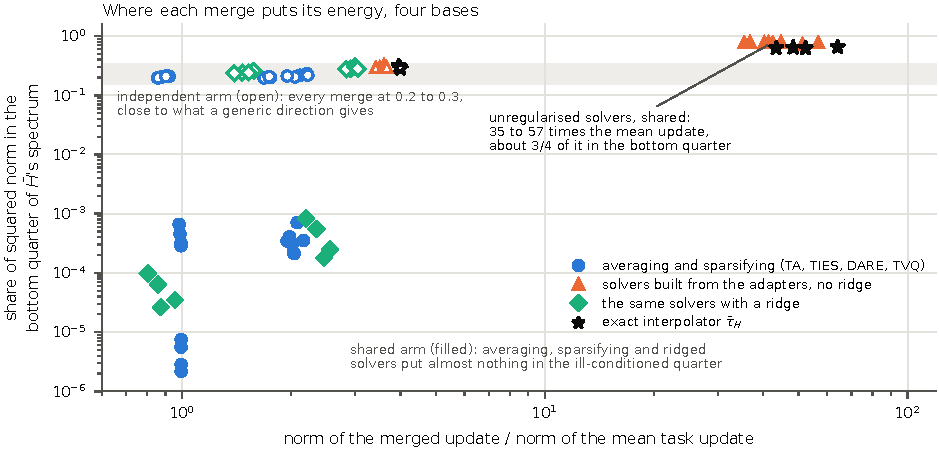
\includegraphics[width=\textwidth]{nc/figures/fig4_mechanism.pdf}
\caption{Where each merged solution puts its energy, on the four bases. Each
point is one method on one base; filled markers are the shared cohort, open
markers the independent one. Horizontal: norm of the merged update relative to
the mean task update. Vertical: share of its squared norm in the bottom quarter
of $\bar H$'s spectrum, the ill-conditioned directions. ``The same solvers with
a ridge'' are adapter-only RegMean at $\lambda = 0.13$ and our encoder at its
selected $\lambda$.}
\label{fig:mechanism}
\end{figure}

For the other methods the mechanism can be checked without any forward pass,
because every merge is arithmetic on the adapter factors
(Figure~\ref{fig:mechanism}). On the shared arm, every averaging and
sparsifying merge has a norm $0.98$ to $2.16$ times that of the mean task
update. The share of its energy in the bottom quartile of $\bar H$'s spectrum
rounds to $0.000$. The two unregularised solvers built from the adapter
factors have norms $35$ to $57$ times the mean update and put $73$ to $80\%$
of their energy there. Among these methods they are the only ones that enter
the ill-conditioned directions, and a ridge brings them back down beside the
heuristics. On the independent arm every method puts $0.19$ to $0.32$ of its
energy in the bottom quarter, close to what a direction unrelated to the
spectrum gives. WUDI is the exception to this picture
(\S\ref{subsec:wudi}): it is amplified on the shared arm without
concentrating in those directions.

\subsection{The other methods}\label{subsec:results}

\begin{table}[pos=tbp]
\centering
\small
\caption{Which merges the collapse reaches. Each method is compared with itself
on shared and independent cohorts, three per arm on four bases. NLL is the
ratio of worst-task excess, shared over independent, over the four bases.
Accuracy is GSM8K exact match and HumanEval pass@1; for MaTS it uses one cohort
per arm. KnOTS is its TIES variant, and diagonal Fisher uses the squared update
as a data-free proxy for the Fisher. The prediction was registered before any
of the methods we did not build was run.}
\label{tab:exposure}
\setlength{\tabcolsep}{3.5pt}
\begin{tabularx}{\textwidth}{>{\raggedright\arraybackslash}p{2.5cm}
                >{\raggedright\arraybackslash}p{1.7cm}
                >{\raggedright\arraybackslash}p{1.5cm}
                >{\raggedright\arraybackslash}X
                >{\raggedright\arraybackslash}X}
\toprule
method & matrix built from & predicted & NLL, shared / indep. & accuracy \\
\midrule
task arithmetic, TIES, DARE, TVQ, KnOTS & no matrix & immune
  & no effect in 15 of 20 cells; largest $0.015$ nats
  & equivalent within $3$ points (GSM8K) and $5$ (HumanEval) \\
\addlinespace
RegMean, activation Grams & data & immune & $0.99$ to $1.14$
  & equal in 8 of 8 cells \\
MaTS & data (Fisher) & immune & $0.93$ to $0.99$
  & equal in 7 of 8; 1 favours shared \\
diagonal Fisher & task updates, diagonal & immune & $0.96$ to $1.08$ & not run \\
\addlinespace
TSV-M (whitening) & task updates & exposed & $0.81$ to $1.19$, mixed sign
  & no cell past the gate \\
\addlinespace
WUDI, as published & task updates & protected by its optimiser & $4.7$ to $47.6$
  & GSM8K $0.00$ to $0.48$ vs.\ $0.25$ to $0.72$ \\
WUDI, closed form & task updates & exposed & $5.3$ to $65.1$
  & GSM8K $0.00$ to $0.18$ vs.\ $0.27$ to $0.72$ \\
\addlinespace
RegMean, adapter-only & adapter factors & exposed & $1.8$ to $65.6$
  & GSM8K $0.00$ to $0.17$ vs.\ $0.29$ to $0.72$ \\
our encoder & adapter factors & exposed & $2.8$ to $76$
  & Mistral $0.000$ on both \\
\bottomrule
\end{tabularx}
\end{table}

\begin{figure}[pos=tbp]
\centering
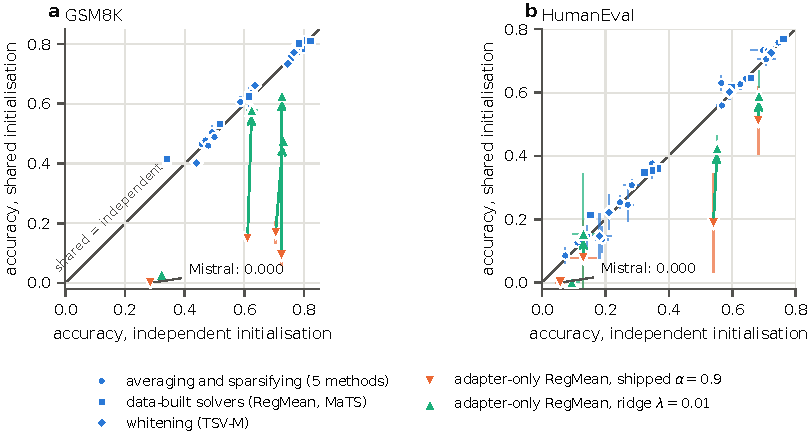
\includegraphics[width=\textwidth]{nc/figures/fig5_accuracy.pdf}
\caption{Downstream accuracy on shared against independent cohorts. Each point
is one method on one base model, the mean over three cohorts per arm, with bars
of one standard deviation across cohorts. Points on the diagonal are unaffected
by the initialisation. Every published method shown lies on or near it;
adapter-only RegMean at its shipped setting ($\alpha = 0.9$) lies far below it.
Arrows go from that setting to the same solver with a ridge of
$\lambda = 0.01$ on the same base, which recovers most of the loss on three
bases and not on Mistral. WUDI is in Table~\ref{tab:wudi}.}
\label{fig:exposure}
\end{figure}

Table~\ref{tab:exposure} and Figure~\ref{fig:exposure} give the outcome for
every method.

\paragraph{Averaging and sparsifying merges are unaffected.} In NLL, $15$ of
$20$ base-by-method cells show no difference that clears the registered gate.
The gate is the larger of $0.005$ nats and twice the standard error, and sits
near $0.01$ nats. The five that do are small and favour the independent arm.
Three of them are the subspace-aligning KnOTS, the heuristic that operates most
directly on subspace geometry. Because a null at hundredths of a nat is weak
evidence, we registered the accuracy comparison as an equivalence test (two
one-sided tests, three cohorts per arm, $240$ cells). All five heuristics are
equivalent across regimes within the registered margins of $3$ points on GSM8K
and $5$ on HumanEval, and each would pass at $0.9$ to $2.0$ points and $2.1$ to
$3.0$ points respectively. The equivalence is a statement about means over the
four bases. One of $40$ cells taken alone exceeds its margin: TIES on Llama at
HumanEval, where the shared arm is $6.5$ points higher.

We also registered that a slight lean towards the shared arm, seen at one
cohort per arm, would vanish at three. It persisted: $29$ of the $38$ non-zero
differences favour the shared arm (sign test, $p = 0.0017$). That test treats
the $40$ cells as independent, although the ten cells of a base share its six
cohorts and its evaluation sets. A permutation test that we ran afterwards,
which relabels whole cohorts within each base, gives $p = 0.007$ for a mean
lean of $0.7$ points, with all four bases leaning the same way. We tested one
explanation in advance. Truncation to rank $r$ discards more of an independent
cohort's merged update: $12$ to $25\%$ of task arithmetic's squared norm,
against $1.3$ to $1.6\%$ on the shared arm, and more on the independent arm for
every heuristic on every base. Merging without truncation should then have
halved the lean. It did not halve on any of the three method-benchmark pairs
where the lean was largest (task arithmetic and DARE at HumanEval, TIES at
GSM8K), so truncation is excluded as its cause. No heuristic enters the
ill-conditioned directions, so the lean is not the solver mechanism either,
and we have no tested explanation for it. In practice, a heuristic merge loses
nothing to a shared initialisation.

\paragraph{Solvers built from data, and a diagonal one, are unaffected.}
RegMean with real activation Grams at its published setting, MaTS with its
blockwise Fisher solved by conjugate gradient, and diagonal Fisher merging were
run on all three cohorts of both arms on all four bases. Our diagonal Fisher
weights each coordinate by its squared update, a data-free proxy, so its matrix
comes from the task updates; being diagonal, it cannot see overlap between
subspaces. The three immunity predictions hold. RegMean shows no effect on any base in either unit and is the most
accurate merge in our experiments on every base; its accuracy on the two arms
agrees within $1.3$ points in all eight base-by-benchmark cells. MaTS shows no
NLL effect, and in accuracy one cell (Mistral, GSM8K) favours the shared arm.
Diagonal Fisher shows one small effect, $1.08$ times on Llama. A practitioner
who has the data RegMean was designed for is unaffected by the collapse.

\paragraph{Whitening is not affected, against our prediction.} TSV-M was
predicted to be exposed. It shows an NLL effect on Mistral only ($1.19$ times),
one in the opposite direction on Yi, and none on Llama and Qwen, and no
accuracy cell clears the gate. The prediction failed. Whitening orthogonalises
the stacked singular vectors rather than solving a least-squares problem in
them, and the rule in \S\ref{subsec:rule} is stated for least-squares merges
alone.

\paragraph{Solvers built from the adapter factors fail.} The data-free form of
RegMean replaces each activation Gram by $A_t^\top A_t$. It is a variant we
constructed, not the published method, and it is the natural choice when only
the adapter files are available. With a minimal ridge ($\lambda = 10^{-6}$) its
worst-task excess (Figure~\ref{fig:ridge}, top row) is $4.1$, $65.6$, $5.8$ and
$1.8$ times larger on the shared arm on Llama, Mistral, Qwen and Yi, and the
gain from tuning the ridge is larger on the shared arm on all four; both match
the registered predictions. In accuracy, with RegMean's own shipped regulariser
($\alpha = 0.9$) and no added ridge, the shared arm scores $0.168$, $0.000$,
$0.148$ and $0.093$ on GSM8K against $0.705$, $0.285$, $0.611$ and $0.724$ on
the independent arm. On Mistral it scores zero on both benchmarks in all three
shared cohorts. A ridge of $\lambda = 0.01$ beats the shipped setting on the
shared arm past the gate on three of four bases on GSM8K, by $31$, $43$ and
$54$ points on Llama, Qwen and Yi, and on two on HumanEval. It does not rescue
Mistral ($0.029$ and $0.002$), whose NLL sweep selects $\lambda = 0.05$, so
$0.01$ is a starting point for a sweep rather than a recommended value.

The second solver of this kind is the closed-form encoder of our earlier
preprint~\citep{pathak2026rd}, which we call \emph{our encoder}. It computes
the exact interpolator $\tauH = \bar D\,\bar H^{+}$ of \S\ref{sec:background}
directly, with an optional ridge on the range of $\bar H$, so it inverts the
collapsed operator itself. Unregularised it is $2.8$ to $76$ times worse on
the shared arm (three cohorts per arm, every base past the gate), and on
Mistral its merged model scores $0.000$ on both benchmarks, recovering to
$0.46$ on GSM8K and $0.24$ on HumanEval with a tuned ridge. The effect
survives with rank truncation disabled, where the ratio grows to $25$ to
$117$: truncating to rank $r$ discards most of the ill-conditioned subspace and
so hides part of the damage. On both solvers, the amount of ridge that is
needed does not track the conditioning, while the amount it buys does; the
selected $\lambda$ is identical across the two arms on three of four bases for
the encoder and on two for adapter-only RegMean.

\paragraph{Numerical precision and truncation.} Both solvers run in float32,
and at $\lambda = 10^{-6}$ and $\lambda = 0$ their systems are badly
conditioned, so the failure could in principle be rounding error. We
registered a check before running it: for each base, arm and solver, recompute
the merge in float64 from the same adapter factors and compare the two after
exact truncation to rank $r$. Precision would be excluded if the median
difference over modules stayed below $1\%$ and the ratio of shared to
independent amplification changed by less than a factor of $2$. The ratios
agree within $0.1\%$ in every case, and $15$ of the $16$ medians are below
$1\%$, at most $0.9\%$. The encoder on the shared Yi cohort is at $1.09\%$ and
fails, so, as registered, we rebuilt that merge in float64 and evaluated it
again. Its worst-task excess is $0.245$ nats against $0.249$ in float32, and
$0.121$ on the independent cohort: rounding does not cause the failure. Runs
we added afterwards show that the float32 merge is unstable instead. The
encoder's per-task bases come from a randomised SVD, and the unregularised
solve amplifies its rounding, so float32 merges that differ only in the random
seed reach worst-task excesses of $0.22$ to $0.28$ nats on this cohort, and
$0.26$ to $0.84$ when the truncation to rank $r$ is exact. All of them lie
above the independent cohort, whose float32 merge agrees with float64 to
$2\times10^{-6}$ in the median over modules. Three draws on a shared cohort of each other base, under the
same seeds, span $0.31$ to $0.33$ nats on Llama, $9.78$ to $9.86$ on Mistral and
$0.19$ to $0.22$ on Qwen. On every base each draw lies above the independent
cohort, and the spread is smaller than the gap to it, most narrowly on Yi
($0.063$ against $0.095$). The float32 values we report for the unregularised
encoder on shared cohorts are single draws of this kind: their direction does
not depend on the draw, but their size moves by $0.02$ to $0.08$ nats, which we
measured on one shared cohort per base. Adapter-only RegMean agrees with
float64 to within $1\%$ on every module.

Every merge in this paper is cut to rank $r$ by a randomised SVD that computes
$r$ vectors with four power iterations and no oversampling. On the merges of
the two solvers it keeps $98.8$ to $99.9\%$ of the norm of the exact
truncation but not its directions: it is a median $30$ to $38\%$ from the exact
rank-$r$ truncation in relative Frobenius norm on the shared arm, and $12$ to
$20\%$ on the independent arm. Both arms are cut the same way, and the
encoder's failure survives with this step removed, as above.

\subsection{Why RegMean's shipped regulariser does not fix it}\label{subsec:default}

RegMean scales the off-diagonal entries of each Gram by $\alpha$, default
$0.9$, which, up to an overall factor of $\alpha$ that cancels in the solve,
is equivalent to adding $\frac{1-\alpha}{\alpha}\operatorname{diag}(G)$: a
shrinkage whose size is set by the scale of the data, not by the conditioning.
It was designed for activation Grams, and we apply it here outside that use.
On the adapter Grams it has the average size of an isotropic ridge of
$5.8\times10^{-4}$ to $6.8\times10^{-4}$, the same on both arms to within
$0.5\%$ (Figure~\ref{fig:ridge}, bottom row). On the independent
arm that dose leaves a condition number of $1.2\times10^{3}$ to
$1.4\times10^{3}$. On the shared arm it leaves $6.6\times10^{3}$ to
$9.1\times10^{3}$, where $\lambda = 0.01$ brings the same layers to about
$1.5\times10^{2}$. The shipped setting applies one dose whatever the regime,
which is ample on a separated cohort and an order of magnitude too small on a
collapsed one, and nothing in the method signals the difference. A user can
lower $\alpha$; the default does not.

\begin{figure}[pos=tbp]
\centering
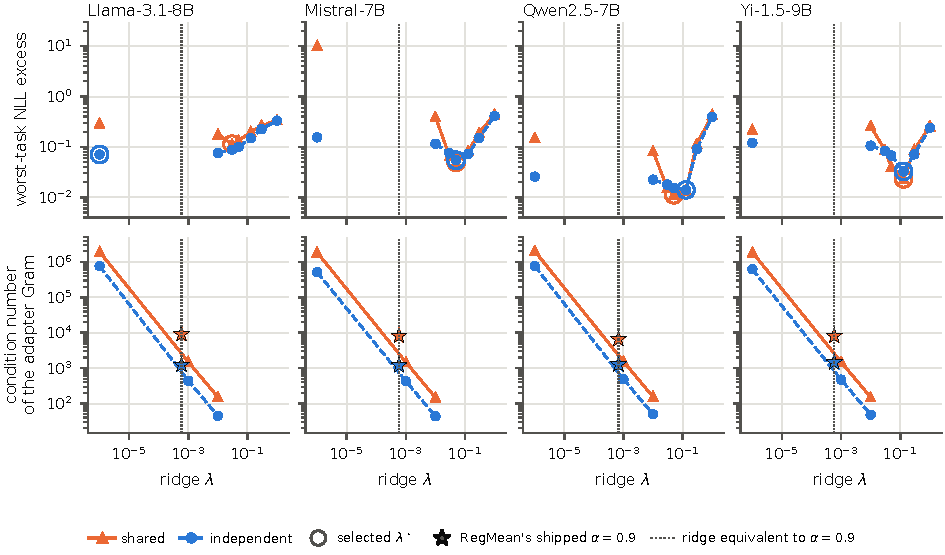
\includegraphics[width=\textwidth]{nc/figures/fig6_ridge.pdf}
\caption{Adapter-only RegMean against an added isotropic ridge $\lambda$, per
base model, on one shared and one independent cohort. \textbf{Top:} worst-task
NLL excess; circles mark the selected $\lambda^\star$, and the point at
$\lambda = 10^{-6}$ is not joined to the rest because no grid point lies
between. \textbf{Bottom:} condition number of the adapter Gram. Stars mark
RegMean's shipped $\alpha = 0.9$, placed at the isotropic ridge of the same
average size, $(1-\alpha)/\alpha$ times the mean diagonal of the Gram (dotted). That
size is the same on both arms, and on the shared arm it leaves a higher
condition number than an isotropic ridge of that size would.}
\label{fig:ridge}
\end{figure}

\subsection{A vision model, and all four tasks}\label{subsec:beyond}

\paragraph{A vision model.} We repeated the central comparisons on CLIP
ViT-B/32 with eight image classification tasks (SUN397, Cars, RESISC45,
EuroSAT, SVHN, GTSRB, MNIST and DTD). We trained rank-$16$ adapters in three
shared and three independent cohorts, merged them as dense updates without
truncation, and scored mean top-1 accuracy over the eight tasks. Every
registered prediction holds. The shared cohorts sit at median cosine $0.96$
and the independent ones at $0.11$. Adapter-only RegMean at
$\lambda = 10^{-6}$ scores $0.043$ on shared cohorts against $0.369$ on
independent ones, and at RegMean's shipped $\alpha = 0.9$ it scores $0.049$
against $0.398$. A ridge of $\lambda = 0.1$, the best grid value on both arms,
repairs it ($0.735$ against $0.747$). Task arithmetic ($0.742$ against
$0.739$) and TIES ($0.721$ against $0.711$) are equivalent within two points.
Activation-Gram RegMean ($0.768$ against $0.770$) and TSV-M ($0.654$ against
$0.670$) show no effect past the gate. WUDI's closed form fails as it does on
language models, $0.045$ against $0.369$. Published WUDI does not fail here.
Shared cohorts merge \emph{better} with it, $0.454$ against $0.358$, a
difference well past the gate and in the opposite direction to the language
models. Our registration asked only for the absence of harm, so this outcome
satisfies it. We did not predict a reversal, however, and cannot explain it,
and it is the clearest open question in this paper about the exposed class.

\paragraph{All four tasks.} The accuracy results so far cover mathematics and
code. We registered tests on the other two tasks: WMT19 English-to-German
(chrF on $500$ pairs) and IFEval (strict prompt-level accuracy on $300$
prompts). They use the seed-1 and independent-1 cohorts and our encoder, whose
merges at $\lambda = 0$ and at the selected $\lambda^\star$ were already
evaluated on the other tasks. On translation the collapse is visible. On the
shared cohort the selected ridge beats $\lambda = 0$ by $13.9$, $55.1$, $2.9$
and $6.5$ chrF points on the four bases, past the gate of $2$ on all four,
while task arithmetic and TIES differ across arms by at most $1.1$ points. On
IFEval it is not visible. The ridge gains $0.080$, $0.333$, $0.043$ and
$0.040$, past the gate on Mistral only; Llama misses by $0.001$ and is counted
as a miss, as registered. The heuristics again differ by at most $0.057$,
inside every gate. The reference rows account for part of this. The
instruction adapter alone does not beat the base model on IFEval on three of
four bases (Llama scores $0.627$ against the base model's $0.703$), so there
is little task skill for a broken merge to lose. The translation adapter is
also below the base model on chrF on three bases, the data-loading defect of
\S\ref{subsec:setup}. What the unregularised merge destroys on translation is
therefore mostly the base model's own ability to translate.

\subsection{Setting the ridge without data}\label{subsec:lambda}

A ridge repairs both solvers built from the adapter factors on most bases,
but the amount needed does not track the conditioning. We tested three data-free rules for choosing it, and all three
failed. The first sets $\lambda$ to bring the adapter Gram to a target
condition number, chosen in advance and evaluated only on unseen cohorts. It
was worse than a fixed $\lambda = 0.01$ on every collapsed cohort tested. On
separated cohorts it met its registered criterion of doing no harm on $4$ of
$6$, the two misses being cohorts where it did better than the minimal ridge,
and on collapsed public cohorts it brought the solver within $1.5$ times task
arithmetic's excess on $2$ of $6$, against a registered $80\%$. The fixed
$\lambda = 0.01$, registered to do the same on at least $80\%$ of collapsed
public cohorts, did so on $1$ of $6$.
Adapter-only RegMean is a ridge regression whose samples and targets can both
be read off the adapter files, so the classical parameter-choice rules apply as
they stand, and we registered generalised cross-validation (GCV) and the
L-curve. Neither repaired the collapse on more than one base of four, and
neither passed any of its three other registered criteria (no worse than
$\lambda = 0.01$, near the best of the sweep, no harm on separated cohorts);
GCV raised the independent cohort's excess on Llama from $0.07$ to $0.19$. GCV
chose $\lambda$ near $10^{-4}$ on shared cohorts and left the worst-task
excess at $1.13$, $8.66$, $0.22$ and $0.45$, against $0.11$, $0.05$, $0.01$
and $0.02$ at the best $\lambda$ of the sweep. On Llama, Qwen and Yi that is
worse than the minimal ridge. The L-curve found no interior corner: on every
base and arm its median choice was $1.3\times10^{-8}$, at the lower edge of a
grid that starts at $10^{-8}$. A data-free way to set the ridge
remains open. We recommend starting at $0.01$ and sweeping on held-out data.

\subsection{Public cohorts}\label{subsec:against}

\paragraph{On public cohorts the solver fails in both regimes.} We merged the
public cohorts that a fixed rule selected (causal language models of at most
$15$B parameters that load without custom code, members sharing rank and
target modules): seven collapsed and thirteen separated, of which one
collapsed cohort could not be loaded. Since public adapters rarely ship their
data, the consequence measure scored each adapter's own greedy completions on
a fixed prompt set under the merged model. Unregularised adapter-only RegMean
at least doubles task arithmetic's excess on $5$ of $6$ collapsed cohorts and
also on $11$ of $13$ separated ones (Fisher's exact test, $p = 0.78$). The
solver fails often on public cohorts, but not more often when they are
collapsed. These merges therefore show how common the collapse is
(\S\ref{sec:prevalence}), not what it costs on public cohorts.

\paragraph{Two candidate causes, tested on our own cohorts.} Public cohorts
differ from ours in ways a fixed rule cannot control, so we injected each
difference into our separated cohorts on Llama and Qwen. A LoRA update is
unchanged when $A$ is multiplied by $4$ and $B$ divided by $4$, but $A^\top A$
is not. That rescaling changes adapter-only RegMean's excess by at most $4\%$,
below the gate, so this factorisation freedom is not the cause, and putting
every adapter in a balanced form changes nothing either. Scale mismatch does
matter, which we did not predict. Making one adapter's update $4$ times larger
multiplies RegMean's excess by $3.9$ and $5.3$ on the two bases, while task
arithmetic's excess falls to $0.26$ and $0.29$ of its unperturbed value. Scale
mismatch between adapters is therefore a hazard specific to solvers, which we
observed on separated cohorts. It does not explain the public data, however: the spread of $A$ norms within a cohort is no larger where the
solver failed than where it did not. The public failures remain unexplained.

\subsection{The rule}\label{subsec:rule}

Across twelve methods, ten of them published methods we did not build, the
collapse reaches exactly the merges that solve a least-squares problem, in
closed form or by gradient descent, whose matrix is built from the adapters
alone: from their factors, or from the task updates they define. That class
includes a published method run exactly as its authors run it. The collapse
does not reach averaging or sparsifying merges, solvers whose matrix is built
from data, a diagonal solver, or whitening.
